
% Assessing the Impact of Label-flipping Attacks
% ------------------------------------------------------------------------------

\section{Assessing the Impact of Label-Flipping Attacks}

\begin{frame}
  \sectionpage

  \fcitefootnote{lavaur_ares_bass_2024}
\end{frame}


\begin{frame}{The Problem of Poisoning Attacks}

  \begin{figure}
    \centering
    \foreach \i in {1,...,5}{%
      \includegraphics<\i>[width=.75\textwidth]{figures/assessment/poisoning/\i.pdf}%
    }
    \caption{Poisoning attacks on FL.}
  \end{figure}

\end{frame}

\begin{frame}{Types of Poisoning Attacks}
  \vspace{1em}
  
  \setlength{\leftmargini}{5pt}
  \begin{tcbraster}[raster columns=2, raster equal height, raster column skip=2em, raster row skip=2em]
    \pause
    \begin{taxobox}[By \emph{component}]
      \begin{itemize}
        \item Data poisoning (\eg, \textbf<5>{label-flipping}, clean-label)
        \item Model poisoning (\eg, gradient boosting)
      \end{itemize}
    \end{taxobox}
    \pause
    \begin{taxobox}[By \emph{objective}]
      \begin{itemize}
        \item Untargeted: impact model performance
        \item Targeted: modify behavior for specific samples
      \end{itemize}
    \end{taxobox}
    \pause
    \begin{taxobox}[By \emph{timing}]
      \begin{itemize}
        \item one-shot: performed once
        \item \textbf<5>{incremental/continuous}: at each round
      \end{itemize}
    \end{taxobox}
    \pause
    \begin{taxobox}[By \emph{proportion}]
      \begin{itemize}
        \item Single attacker
        \item Colluding attackers: multiple coordinated participants
      \end{itemize}
    \end{taxobox}
  \end{tcbraster}
\end{frame}
  

\begin{frame}{Scope of the Study}
  % \begin{block}{Our work\normalfont~\cite{lavaur_ares_bass_2024}}
  %   Continuous label-flipping attacks in an collaborative intrustion detection context.
  % \end{block}
  \textbf{Existing studies}
  \begin{itemize}
    \item Often partial, focusing on challenging a specific defense mechanism.
    \item Lack of reproducibility and comparability (different datasets, models, and attacks).
    \item No targeted attacks binary classification.
  \end{itemize}

  \pause
  \textbf{Research Questions}
  \begin{enumerate}
    \item Is the behavior of poisoning attacks predictable?
    \item Do hyperparameters influence the impact of poisoning attacks?
    \item Are IDS backdoors realistic using label-flipping attacks?
    \item Is there a critical threshold where label-flipping attacks begin to impact performance?
    \item \alert<3>{Is gradient similarity enough to detect label-flipping attacks?}
  \end{enumerate}
\end{frame}

% \begin{frame}{Experimental Setup}

%   \textbf{Sound experiments}~\cite{uetz_ReproducibleAdaptableLog_2021,ACM_artifacts}:
%   \begin{itemize}
%     \item \emph{valid} (i.e., well-defined and unrefutable);
%     \item \emph{controllable} (e.g., parameterized); and
%     \item \emph{reproducible} (i.e., the same results can be obtained by another group using the author’s artefact).
%   \end{itemize}

% \end{frame}

% \begin{frame}{Experimental Setup}
    
%   Experiment orchestration using \texttt{Eiffel}~\cite{lavaur_icdcs_demo_2024}.
%   \begin{itemize}
%       \item \texttt{Flower} simulation framework~\cite{beutel_Flowerfriendlyfederated_2020} for \gls{fl}.
%       \item \texttt{Hydra} for experiment generation and configuration.
%       \item Custom-made poisoning engine with different attack strategies.
%       \item Nix~\cite{dolstra_purelyfunctionalsoftware_2006} and Poetry to fix system and Python dependencies, enabling reproducibility.
%   \end{itemize}

%   1,067 experiments $\times$ 10 seeds (1,613 hours of computation.)
% \end{frame}


% \begin{frame}{RQ1: Are Poisoning Attacks Predictable?}

%   \begin{figure}
%     \centering
%     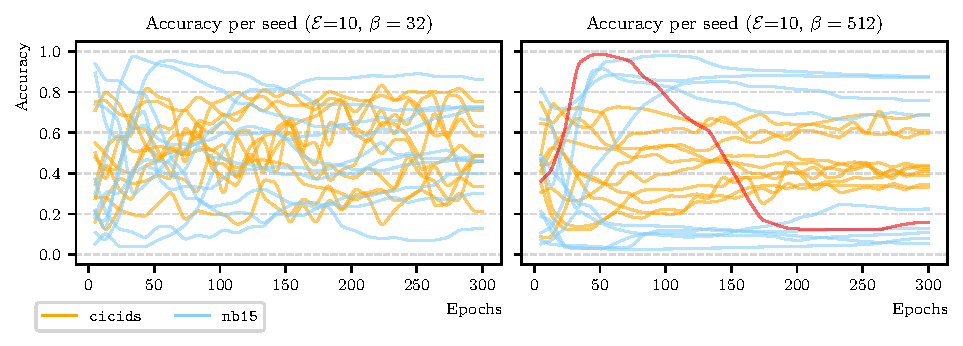
\includegraphics[width=.8\textwidth]{figures/assessment/accuracy_per_seed.pdf}
%     \caption{Predictability of label-flipping attacks.}
%   \end{figure}

%   \begin{itemize}
%     \item Very high variance in the results, but tends to stabilize (on different values) after a few rounds.

%     \item The impact of the attack is highly dependent on the seed.
%     \begin{itemize}
%       \item[$\rightarrow$] Initial parameters, data shuffling, partitioning, \dots
%     \end{itemize}
%   \end{itemize}


% \end{frame}

% \begin{frame}{RQ2: Do Hyperparameters Influence the Impact of Poisoning Attacks?}

%   \begin{figure}
%     \centering
%     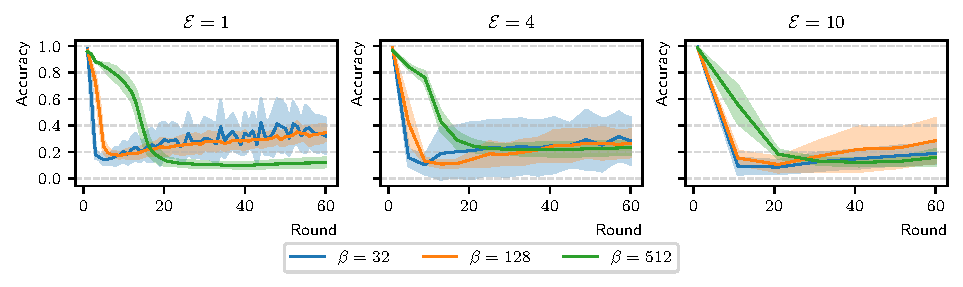
\includegraphics[width=\textwidth]{figures/assessment/hyperparams-late-icdcs.pdf}
%     \caption{Effect of the hyperparameters on the accuracy of the poisoned
%     model in the late scenario (50\% attackers, CICIDS).}
%   \end{figure}

%   \begin{itemize}
%     \item \texttt{late-3} scenario: attackers start poisoning after 3 rounds
%     \item High batch size leads to more inertia, less instantaneous impact
%     \begin{itemize}
%       \item[$\rightarrow$] More impactful in constrained environments
%     \end{itemize}
%   \end{itemize}

% \end{frame}

\begin{frame}{RQ5: Is Gradient Similarity Enough to Detect Label-Flipping Attacks?}

  \begin{columns}
    \begin{column}{.45\textwidth}
      \begin{itemize}
        \item Known technique to detect poisoning attacks~\autocite{tolpegin_DataPoisoningAttacks_2020}.
        \item Higher heterogeneity makes it harder to detect attackers.
        \item Colluding attackers usually form a cluster of their own.
      \end{itemize}
    \end{column}
    \begin{column}{.55\textwidth}
      \begin{figure}
        \centering
        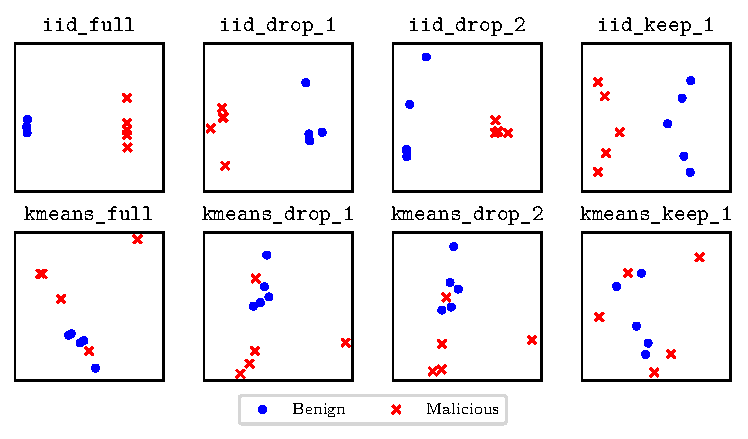
\includegraphics[width=\textwidth]{figures/assessment/similarity-untargeted-colluding-cicids.pdf}
        \caption{PCA projection of the uploaded gradients in 2D (CICIDS).}
      \end{figure}
    \end{column}
  \end{columns}

  \fcitefootnote{tolpegin_DataPoisoningAttacks_2020}

\end{frame}

\begin{frame}{Takeaways}

  A \emph{deeper} understanding of the behavior of label-flipping attacks in FL-based CIDSs.
  \begin{itemize}\small
    \item Unpredictability.
    \item Hyperparameter dependencies, but not on the average performance impact.
    \item Limited by the models' generalization capabilities and the characteristic overlap between classes.
    \item Proximity-based detection techniques show limitations in detecting poisoning attacks.
  \end{itemize}
  
  \onslide<2>{A \alert{reproducible} evaluation framework to study the impact of label-flipping attacks in FIDS
using FL.
  \begin{itemize}\small
    \item Reproducible, extendable, and available in open-access\footnote<2>{https://github.com/leolavaur/eiffel}.
    \item Calls to be extended to other poisoning attacks, datasets, and partitioning strategies.
  \end{itemize}}
\end{frame}

% \begin{frame}{Future Work}

%   \begin{enumerate}    
%     \item Extending the framework
%     \begin{itemize}
%       \item More datasets (currently CICIDS and UNSW-NB15).
%       \item More attack strategies, \eg, backdoors.
%       \item Imrove documentation and usability for other researchers.
%     \end{itemize}

%     \item Deeper heterogeneity study with more realistic assumptions.
%     \begin{itemize}
%       \item Meaningful dataset partitioning.
%       \item Cross-dataset knowledge transfer.
%       \item Leveraging independently generated datasets.
%     \end{itemize}

%   \end{enumerate}

% \end{frame}